\section{Results}

\subsection{Distinctiveness}

%\begin{figure*}[t]
%\centerline{% 
%		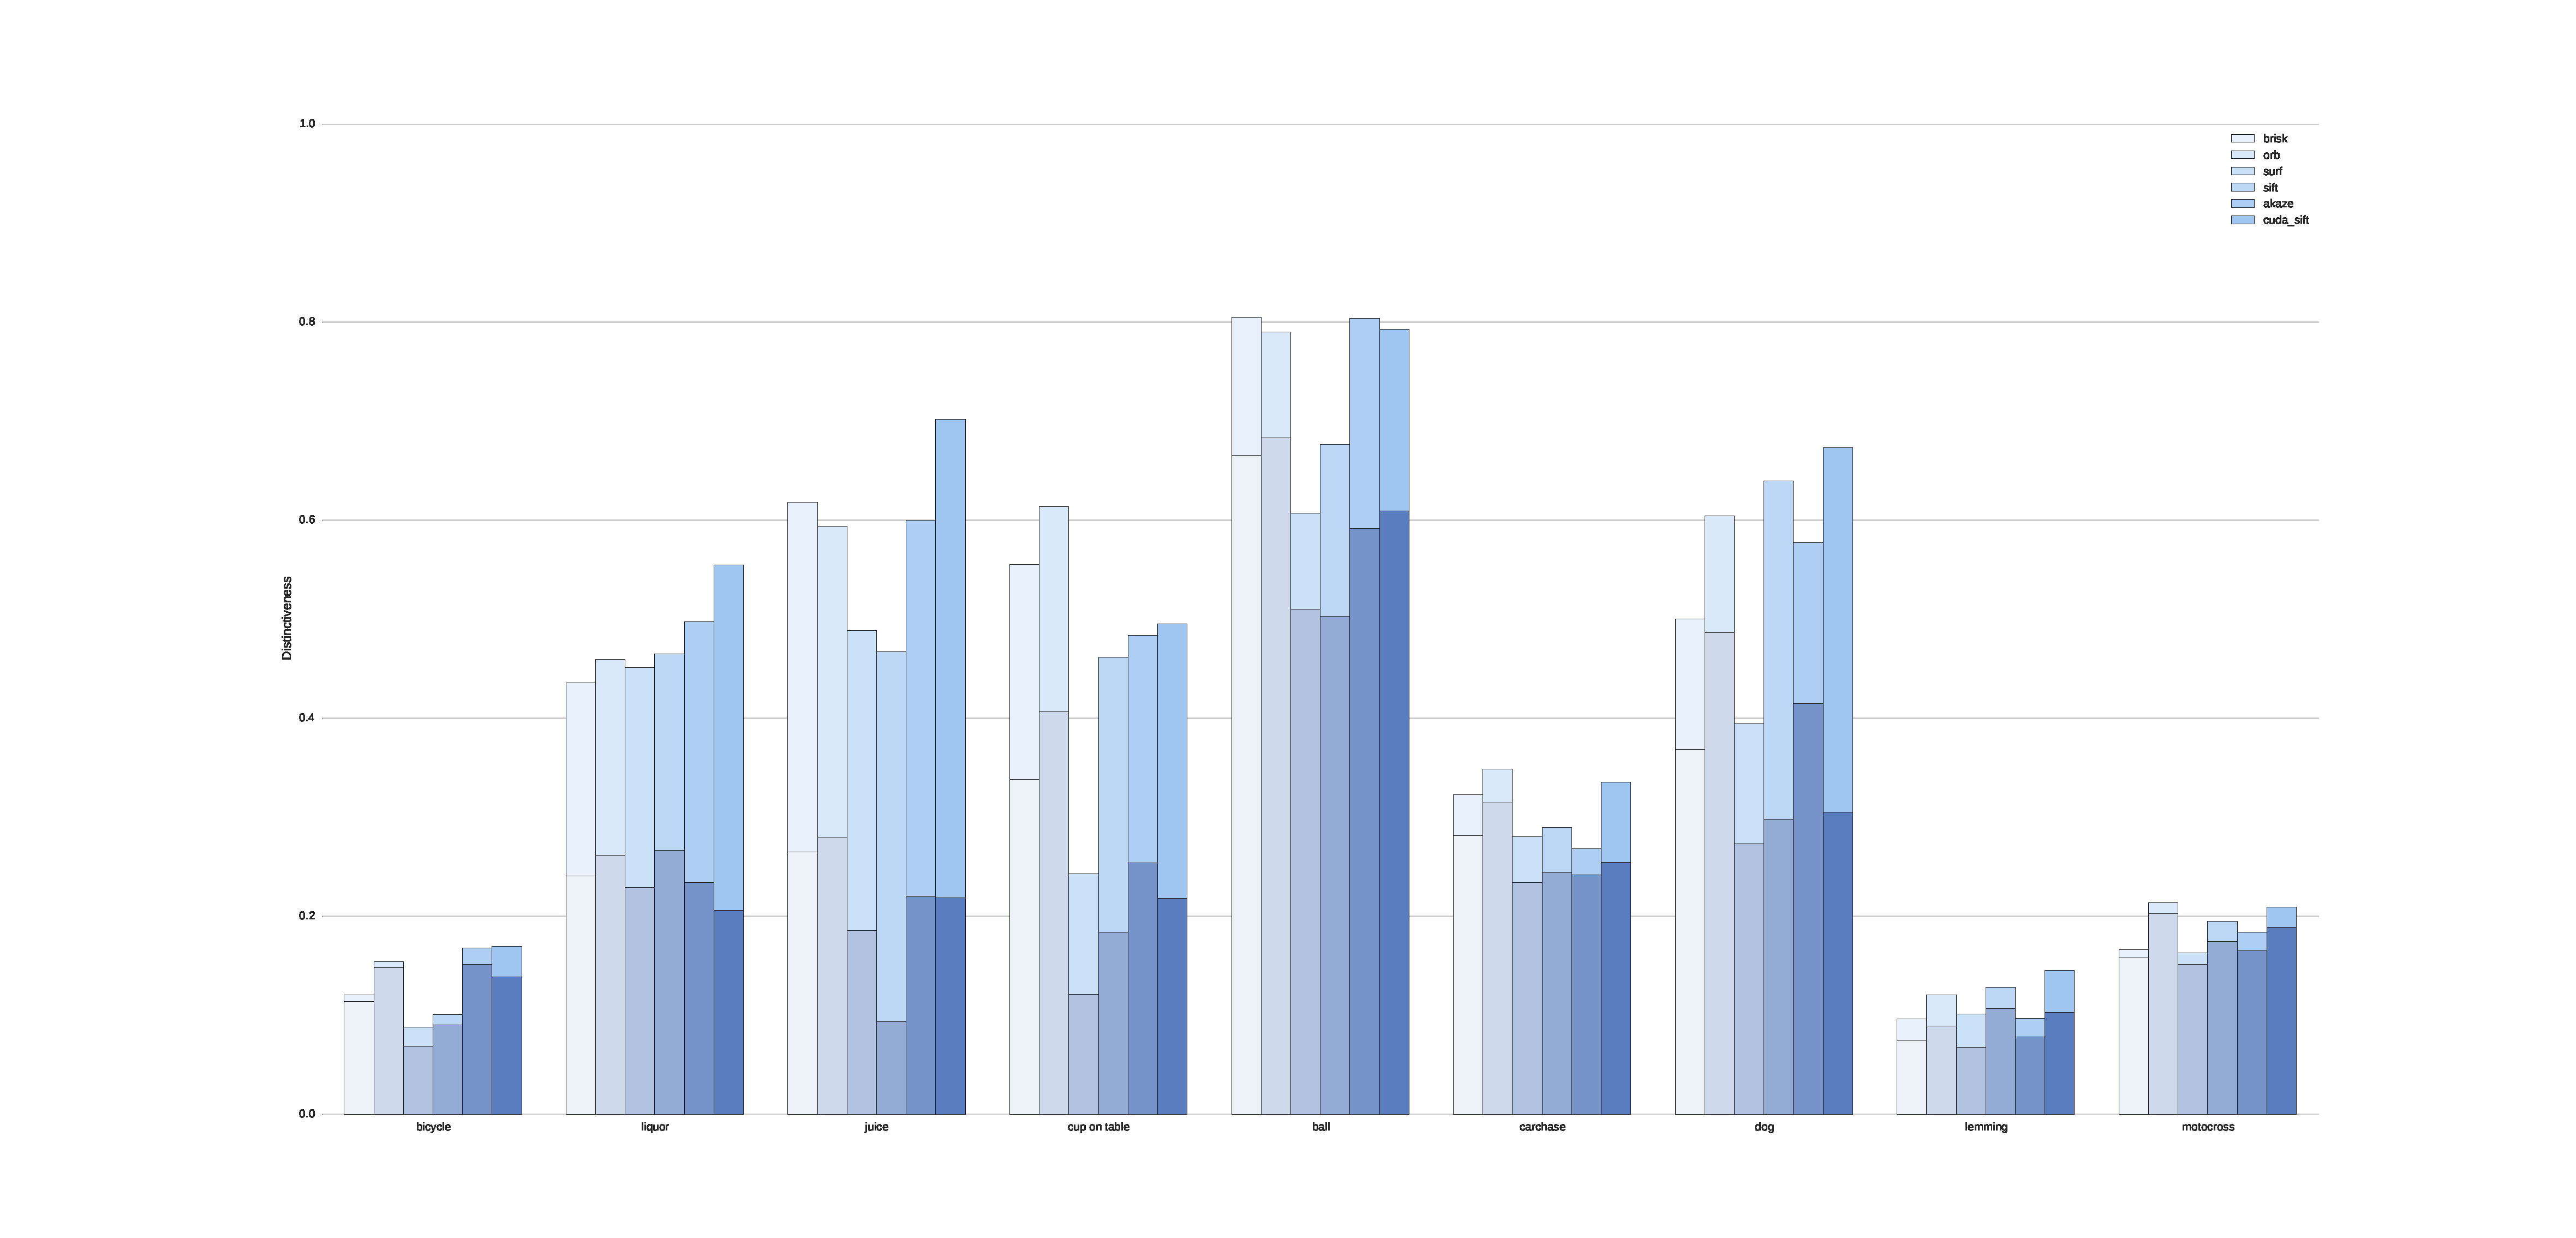
\includegraphics[width=0.98\linewidth]{imgs/distinctivenessTP.pdf}}
%    \vspace{-2mm} 
%	\caption{Examples taken from the dataset showing the ratio of true positives and ambiguous true positives. The lighter color bars show the number of true positives that will actually pass the second best result test.}
%	\label{fig:distinctiveness}
%\end{figure*}

Tab.~\ref{table:tp_ratio} shows the average number of key-points extracted, descriptors belonging to the object to track and the ratio of true positives (TP), false positives (FP) and true positives that pass the second best match ratio check (TTP). It is interesting to notice that BRISK, ORB and SIFT extract a higher number of feature descriptors in general. In particular BRISK and ORB have a higher number of key-points extracted within the area of the object. However, looking at the average amount of true positives it can be seen that the best performing descriptors are AKAZE and the implementation of SIFT on the GPU. This is a first indicator of the quality of the descriptors extracted. Moreover, it can be noticed that the true positives are also more distinctive in the case of AKAZE and SIFT since the number of TTP is higher.

\begin{table}[b]
\caption{Average number of feature extracted, object features, true positives and false positives. Every row is normalized by its maximum value.}
\vspace{-2mm} 
\centerline{% 
		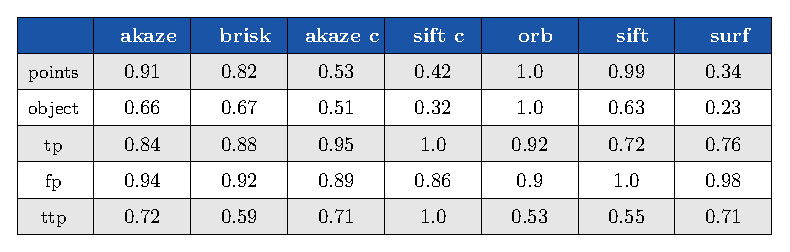
\includegraphics[width=0.98\linewidth]{tables/descriptivness_ratio.pdf}}
    \vspace{-2mm} 
	\label{table:tp_ratio}
\end{table}

\subsection{Tracking accuracy}

\begin{figure}[t]
	\vspace{2mm}
\centerline{%
	\subfigure{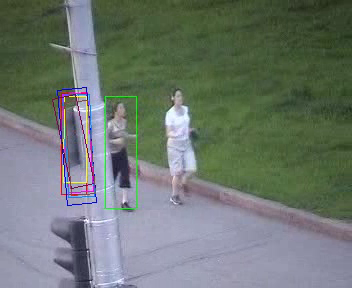
\includegraphics[width=0.48\linewidth]{imgs/results/ex5.png}}
	\subfigure{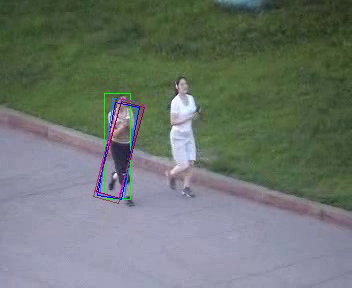
\includegraphics[width=0.48\linewidth]{imgs/results/ex6.png}}}
\caption{Examples showing the behaviour of the feature descriptors upon occlusion. Upon recovery from track loss more descriptive descriptors allow the tracker to recover faster.}
\vspace{-3mm}
\label{fig:tracking_results}
\end{figure}


As explained in the previous section \ref{sec:accuracy}, we evaluated the performance of the feature descriptors running our tracker and calculating the overlap measure for low, medium and high accuracy requirements. Our experiments show that AKAZE, BRISK, ORB and SIFT have comparable results. It is interesting to note that BRISK and ORB compensate their weak distinctiveness with a higher amount of weak descriptors extracted. High numbers of feature points proved to be effective in tracking in the video sequences where the object suffers drastic scale changes and full occlusion, making the recovery after track loss faster (Fig.~\ref{fig:tracking_results}). We also noticed that AKAZE, more than SIFT, suffers the change in scale. Tab.~\ref{table:taccuracy} shows the tracking results on all the video sequences included in the dataset.  



\subsection{Tracking performance}

\begin{figure}[b]
	%\vspace{-2mm}
	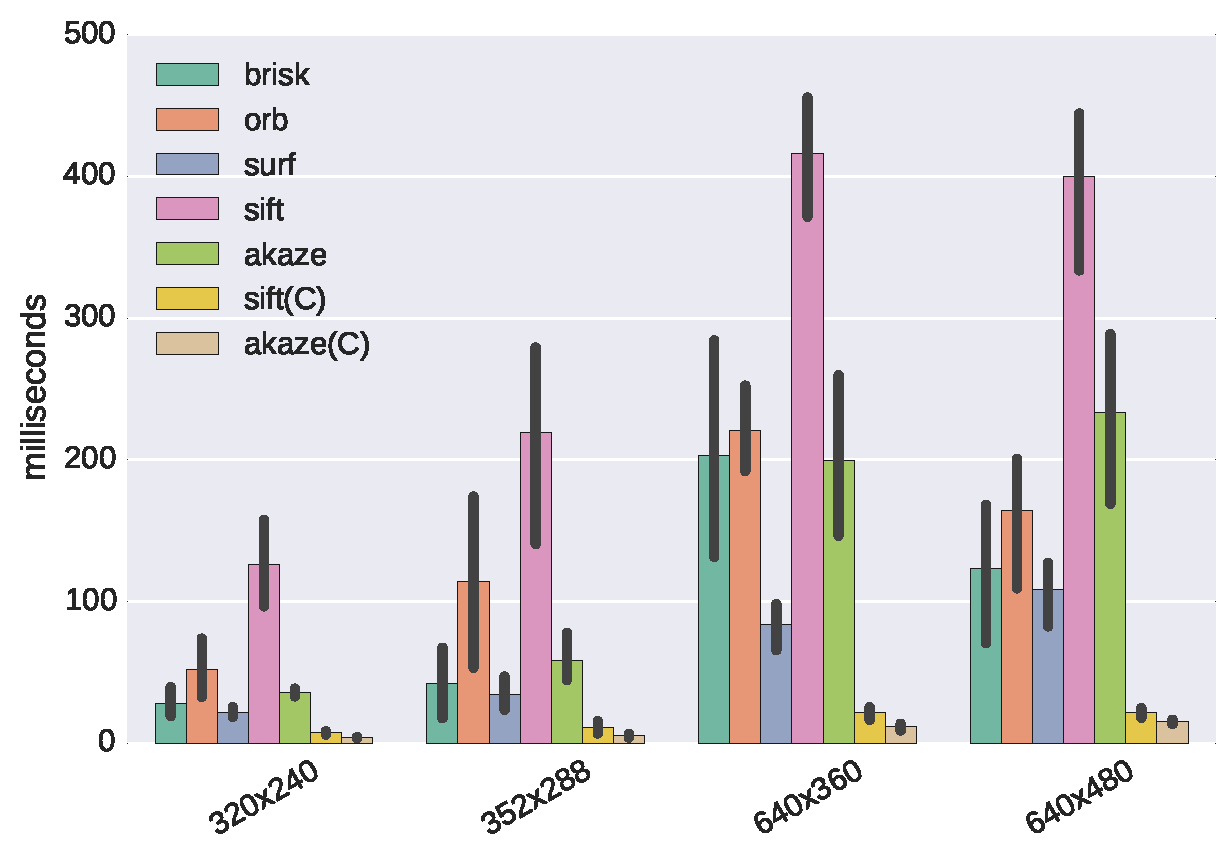
\includegraphics[width=0.95\linewidth]{imgs/tracker_fps_std.pdf}
\vspace{-2.5mm}	
\caption{Average time spent on tracking the object in a single frame. Some important factors are the resolution and the amount of descriptor extracted. The variance of the results are a good indication of how much the quantity of feature descriptor influence the performance. It can be seen that the implementations have a smaller variation due to the high level of parallelism. }
\label{fig:speed}
\end{figure}

The dataset used for benchmarking includes video sequences of various resolution. Fig.~\ref{fig:speed} shows the average performance of each feature descriptor on the resolutions having the highest number of sequences. The two most important factors that influence performances are resolution and number of key points extracted. The first influence particularly the detection step when the scale space of descriptors is computed and key-points are detected, the second influence more the compute step when feature descriptors are calculated and the matching step. the average performance of each separate step can be seen in Fig.~\ref{fig:speed_b}. One interesting thing to notice is the variance of the performance in Fig.~\ref{fig:speed}, BRISK, ORB and SIFT have the broader variance while cuda sift and cuda akaze have the thinner one. This is also a good indicator of the level of parallelism of the implementation of the descriptor.  

%We evaluate the performance of each feature descriptor in three different steps: detection, computation and matching. Fig.~\ref{fig:speed} shows the overall results on the dataset. It is interesting to notice that despite AKAZE exploits multiple core on the CPU, its detection part is expensive due to the non-linear filtering. Brisk and ORB are faster but then the matching step is more expensive given the higher number of features extracted. Please note that this numbers are only informative. We think that it is not fair to compare multi-threaded implementations (e.g AKAZE) with single threaded (SIFT) or GPU implementation (SIFT).

\begin{figure}[t]
	%\vspace{-2mm}
	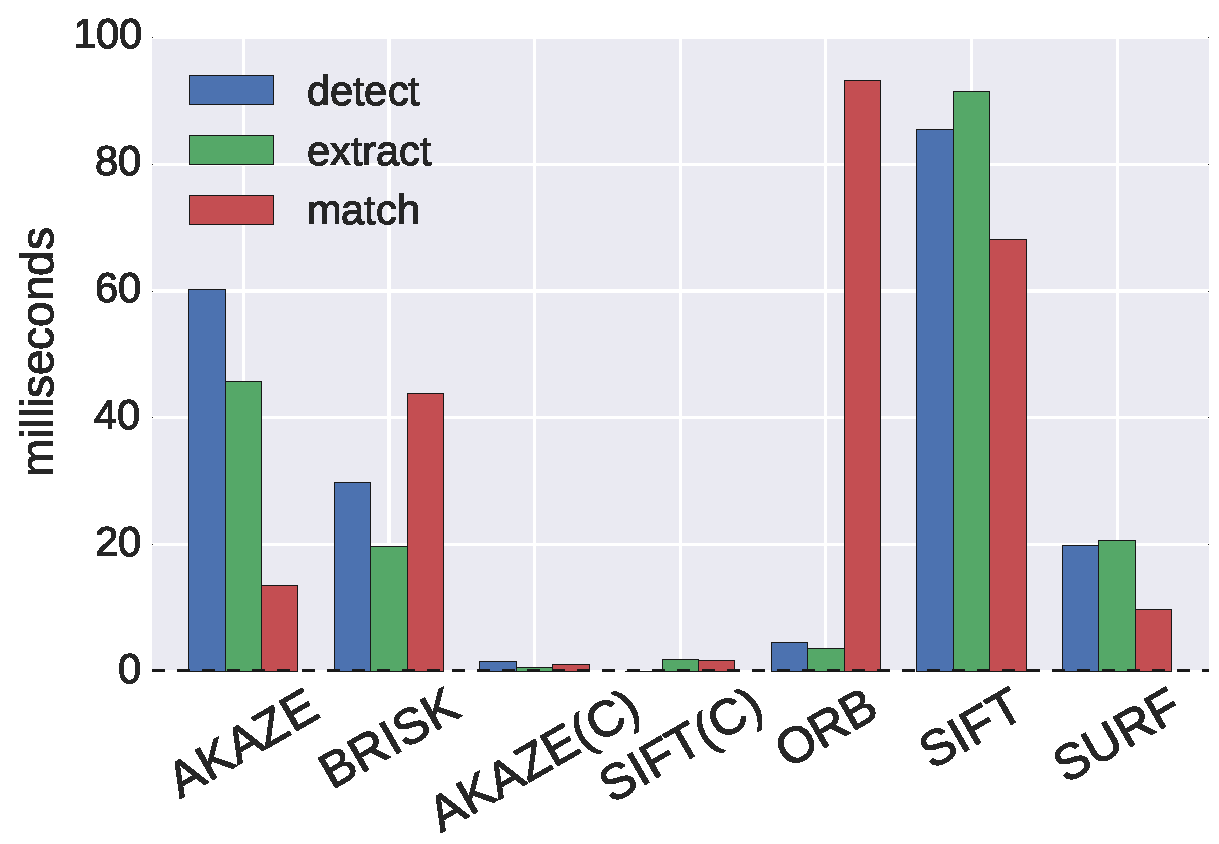
\includegraphics[width=0.95\linewidth]{imgs/performances.pdf}
\vspace{-2.5mm}	
\caption{Performance of the compute,detect and match steps of each feature descriptor.}
\label{fig:speed_b}
\end{figure}

%\begin{table}
%\caption{Average time spent on a single frame by the tracker.}
	%\vspace{-2mm}
%	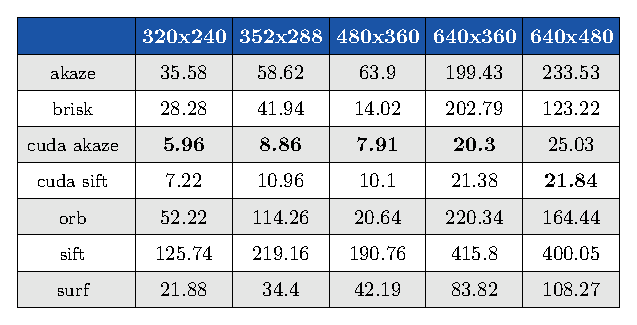
\includegraphics[width=0.95\linewidth]{tables/resolution_times.pdf}
%\vspace{-2.5mm}	
%\label{fig:fps}
%\end{table}

\subsection{Consideration}

Most of the feature descriptors proved to be effective for tracking purposes showing a good precision and performance allowing them to be used in real time frameworks, crucial aspect for robotics. Despite being weak descriptors ORB and BRISK have been proven to be good for real time frameworks but a good trade-off between feature descriptors generated and accuracy has to be defined. AKAZE and SIFT has been proven to be more distinctive descriptors but only their implementations of the GPU allow real time performances. \\
There are still some issue that needs to be addressed in order to have a robust tracking system. First, even if many descriptors are invariant to scale, we noticed that this not hold for drastic scale changes like in Fig.~\ref{fig:tra}. Second, feature descriptors are sensitive to light conditions, Fig.~\ref{fig:trb}, this is particularly relevant for robotics applications since the interaction of a robotic platform with a target object may occlude the source of lighting. Third, the common matching approach to detect an object or compute the transformation between images \cite{mikolajczyk05} does not work in the presence of instances of multiple target with similar appearance, this is the case shown in Fig.\ref{fig:trc} where more players have the same outfit.









